% Roadmap in three horizons with four swimlanes.
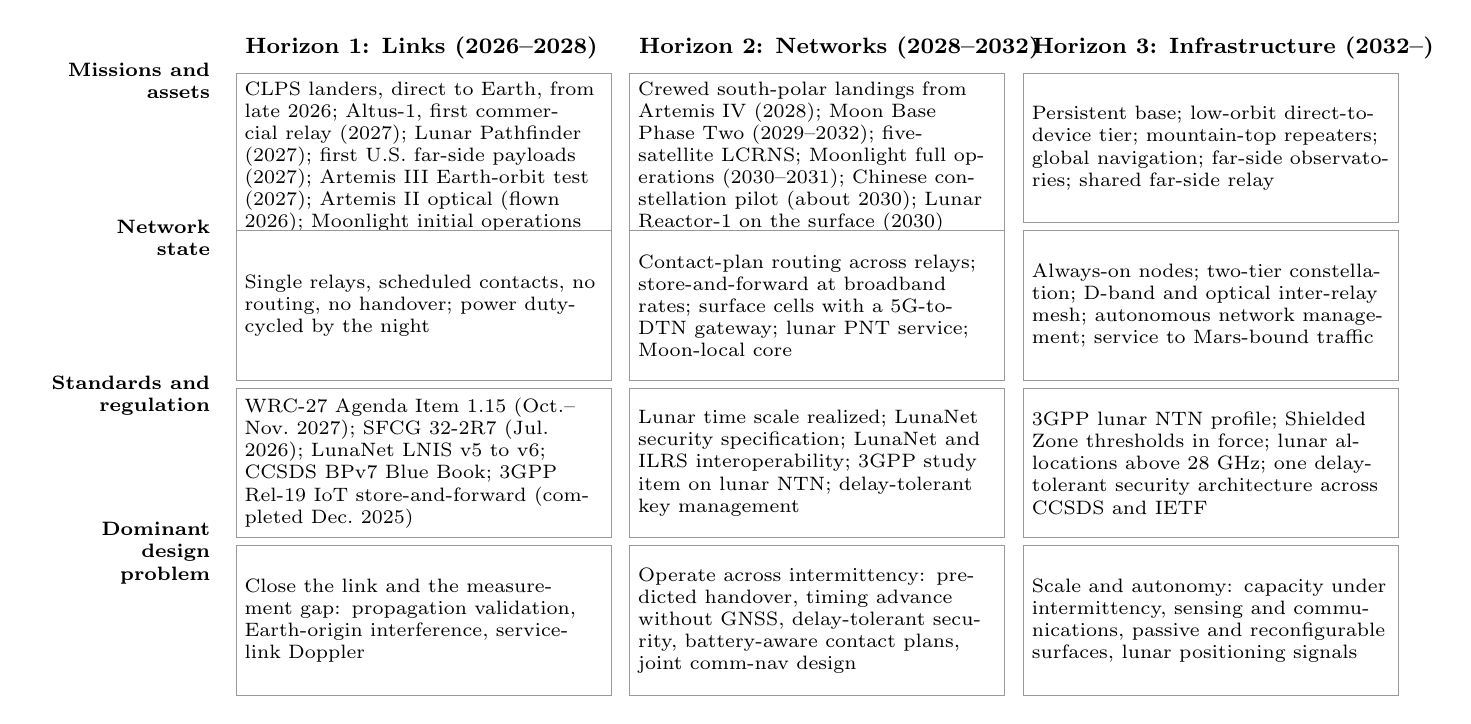
\begin{tikzpicture}[x=1cm,y=1cm,font=\scriptsize,
  cellb/.style={draw=black!40, fill=white, align=left, inner sep=3pt, text width=4.55cm, minimum height=1.9cm, anchor=north west},
  lane/.style={font=\scriptsize\bfseries, anchor=east, align=right, text width=2.2cm},
  hor/.style={font=\footnotesize\bfseries, anchor=south west}]
\node[hor] at (2.5,0.05) {Horizon 1: Links (2026--2028)};
\node[hor] at (7.5,0.05) {Horizon 2: Networks (2028--2032)};
\node[hor] at (12.5,0.05) {Horizon 3: Infrastructure (2032--)};
\node[lane] at (2.3,-0.1) {Missions and\\assets};
\node[cellb] at (2.5,0) {CLPS landers, direct to Earth, from late 2026; Altus-1, first commercial relay (2027); Lunar Pathfinder (2027); first U.S. far-side payloads (2027); Artemis~III Earth-orbit test (2027); Artemis~II optical (flown 2026); Moonlight initial operations (2028--2029)};
\node[cellb] at (7.5,0) {Crewed south-polar landings from Artemis~IV (2028); Moon Base Phase Two (2029--2032); five-satellite LCRNS; Moonlight full operations (2030--2031); Chinese constellation pilot (about 2030); Lunar Reactor-1 on the surface (2030)};
\node[cellb] at (12.5,0) {Persistent base; low-orbit direct-to-device tier; mountain-top repeaters; global navigation; far-side observatories; shared far-side relay};
\node[lane] at (2.3,-2.1) {Network\\state};
\node[cellb] at (2.5,-2.0) {Single relays, scheduled contacts, no routing, no handover; power duty-cycled by the night};
\node[cellb] at (7.5,-2.0) {Contact-plan routing across relays; store-and-forward at broadband rates; surface cells with a 5G-to-DTN gateway; lunar PNT service; Moon-local core};
\node[cellb] at (12.5,-2.0) {Always-on nodes; two-tier constellation; D-band and optical inter-relay mesh; autonomous network management; service to Mars-bound traffic};
\node[lane] at (2.3,-4.1) {Standards and\\regulation};
\node[cellb] at (2.5,-4.0) {WRC-27 Agenda Item 1.15 (Oct.--Nov.\ 2027); SFCG 32-2R7 (Jul.\ 2026); LunaNet LNIS v5 to v6; CCSDS BPv7 Blue Book; 3GPP Rel-19 IoT store-and-forward (completed Dec.\ 2025)};
\node[cellb] at (7.5,-4.0) {Lunar time scale realized; LunaNet security specification; LunaNet and ILRS interoperability; 3GPP study item on lunar NTN; delay-tolerant key management};
\node[cellb] at (12.5,-4.0) {3GPP lunar NTN profile; Shielded Zone thresholds in force; lunar allocations above 28 GHz; one delay-tolerant security architecture across CCSDS and IETF};
\node[lane] at (2.3,-6.1) {Dominant design\\problem};
\node[cellb] at (2.5,-6.0) {Close the link and the measurement gap: propagation validation, Earth-origin interference, service-link Doppler};
\node[cellb] at (7.5,-6.0) {Operate across intermittency: predicted handover, timing advance without GNSS, delay-tolerant security, battery-aware contact plans, joint comm-nav design};
\node[cellb] at (12.5,-6.0) {Scale and autonomy: capacity under intermittency, sensing and communications, passive and reconfigurable surfaces, lunar positioning signals};
\end{tikzpicture}
